\section{Zielsetzung}
In diesem Versuch wird der Effekt der Faraday Rotation verwendet, um die
effektive Masse der Leitungselektronen in n-dotierten Galliumarsenid zu messen.

\section{Theorie}
In diesem Versuch scheint eine linear polarisierte elektromagnetische Welle
durch einen Halbleiter. Dieser Halbleiter wird einem Magnetfeld parallel zur
Lichtausbreitung ausgesetzt, was zu einer Drehung der Polarisationsachse führt.
Die konkreten Prozesse werden im Folgenden beschrieben.

\subsection{Halbleiter \cite[][Kap. 13, 14]{book:expi3}}

Elektronen in Festkörpern haben anstelle von diskret definierten Zuständen
Aufenthaltswahrscheinlichkeiten in der Form von Bändern. Diese Bänder sind eine
direkte Folge der Kristallstruktur des Festkörpers und der periodischen
Potenzialfunktion.
% Ich habe einfach nur ein paar Zeilen zu der Bandstruktur aufgeschrieben.
Die Elektronen füllen nun die möglichen Zustände nach der
Fermi-Dirac-Verteilung auf. Die Bänder oberhalb der Fermi-Energie heißen nun
Leitungsbänder und die unterhalb der Fermi-Energie Valenzbänder. Leitende
Festkörper zeichnen sich durch Elektronen im ungebundenen Zustand aus.
Isolatoren wiederum haben eine große Bandlücke $E_g > 3 \unit{\eV}$
\cite{web:Bandlücke} zwischen den gebundenen Elektronen und dem ersten freien
Leitungsband. Diese Bandlücke ist bei Halbleitern in der Größenordnung von etwa
$\qtyrange{1}{3}{\eV}$\cite{web:Bandlücke}. Die Bandstruktur von Halbleitern
ist auch eine Funktion des Impulses der Elektronen bzw. deren Wellenvektor
$\vec{k}$. Die Energiefunktion, die das Band beschreibt, kann durch eine
quadratische Funktion in $\vec{k}$ angenähert werden (siehe Abbildung
\ref{fig:band}). Elektronen können zum Beispiel thermisch oder optisch angeregt
werden, um vom Valenzband ins Leitungsband zu wechseln. Dazu müssen sie die
nötige Energie erhalten, um die Bandlücke zu überwinden.

% Noch was zum Thema Dotierung?


\begin{figure}
	\centering
	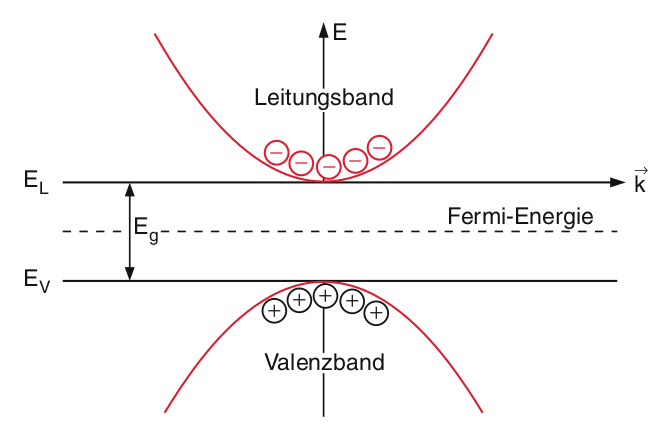
\includegraphics[width=0.8\textwidth]{./Bilder/bandstrukt.png}
	\caption{Die Bandstruktur eines Halbleiters im $k$-Raum\cite{book:expi3}.}\label{fig:band}
\end{figure}

\subsection{Effektive Masse \cite[][Kap. 14]{book:expi3}}

Die effektive Masse ist relevant für die Bewegungsgleichungen der Elektronen im
Leitungsband von Halbleitern sowie der Elektronen Löcher im Valenzband. Sie
kann anstelle der Masse eines freien Elektrons verwendet werden, so können die
Bewegungsgleichungen für freie Elektronen auch in Materie angewendet werden.
Auf ein Elektron oder ein Loch wirkt eine Kraft $\vec{F} = e \vec{E}$ ausgelöst
durch ein elektrisches Feld $\vec{E}$. Es erfährt eine Beschleunigung $\vec{a}
	= \vec{F}/m_e$ und so eine kinetische Energie $E = 1/2 m v²$ mit $v= a\cdot t$.
Zusätzlich erhält das Elektron auch ein ortsabhängiges Potential.

Will man trotzdem die Elektronen im Kristall wie freie Elektronen behandeln,
sodass alle Formeln wie z.B. das Newtonsche Kraftgesetz $\vec{F} = d\vec{p}/dt$
verwendet werden können ist es sinnvoll eine effektive Masse einzuführen
% In einem Minimum des Potenzials kann die Beschleunigung der Elektronen als
Beschreibt man das Elektron durch ein WellenPaket und seine Geschwindigkeit $v$
als Gruppengeschwindigkeit so erhält man
\begin{align}
	\vec{v}_g             & = \frac{d\omega}{d\vec{k}} = \frac{1}{\hbar} \frac{dE}{d\vec{k}} \t{ mit } E = \hbar \omega                        \\
	\intertext{und für die Beschleunigung}
	\frac{d\vec{v}_g}{dt} & = \frac{1}{\hbar} \frac{d²E}{d\vec{k} dt} = \frac{1}{\hbar} \left(\frac{d²E}{d\vec{k}²}\right)\frac{d\vec{k}}{dt}.
	% a = \frac{1}{\hbar²}\frac{d\epsilon}{dk²}q\vec{E}
\end{align}
Für die freie Newtongleichung gilt $\vec{F} = \frac{d\vec{p}}{dt} =\frac{1}{\hbar}\frac{d\vec{p}}{dt} $.
Deshalb ergibt sich eine Gruppenbeschleunigung von
\begin{align}
	\frac{d\vec{v}_g}{dt} = \frac{1}{\hbar²} \left(\frac{d²E}{d\vec{k}²}\right) \vec{F}
\end{align}

So ergibt sich die effektive Masse als
\begin{align}
	m^* & = \hbar^2 \cdot \left(\frac{d²E}{d k_i d k_j}\right)^{-1} .
\end{align}
Im hinreichend symmetrischen Festkörper ist diese Darstellung auch
ohne Tensor Schreibweise annähernd richtig:
\begin{align}
	m^* = \hbar² \frac{dk²}{d²E}
\end{align}

\subsection{Zirkulare Doppelbrechung \cite{man_a}}
\begin{figure}[H]
	\centering
	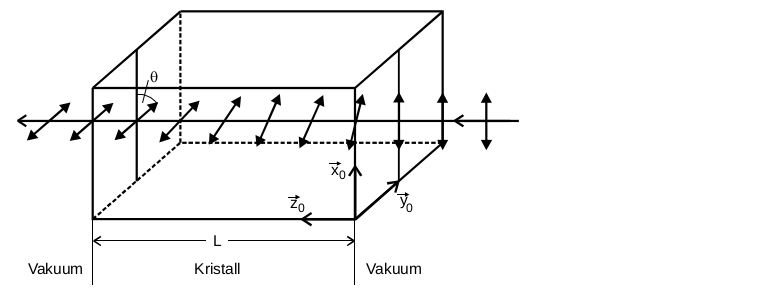
\includegraphics[width=0.8\textwidth]{./Bilder/zirpol.png}
	\caption{Rotation der Polarisationsebene bei zirkularer Doppelbrechung \cite{man_a} }\label{fig:zirpol}
\end{figure}

Es ist möglich linear polarisiertes Licht in eine rechts- und eine
linkszirkular polarisierte Welle zu zerlegen.

\begin{align}
	E(z)    & = \frac{1}{2}(E_R(z) + E_L(z))                   \\
	E_R (z) & = (E_0 \vec{x}_0  - i E_0 \vec{y}_0) e^{i k_R z} \\
	E_L (z) & = (E_0 \vec{x}_0  + i E_0 \vec{y}_0) e^{i k_L z}
\end{align}

Bestimmte Kristalle können so die Polarisationsebene eines Linear polarisierten
Lichtstrahls drehen, da die Brechungsindizes für links und für rechtszirkular
polarisiertes Licht unterschiedlich sind.

Mit den Abkürzungen $ \psi := \frac{L}{2} (k_R + k_L)$ und $\theta :=
	\frac{L}{2} (k_R -k_L)$ ergibt sich für die Polarisationsebene am Ende des
Kristalls mit der Länge $L$
\begin{align}
	E(L) & = E_0 e^{i\psi} (\cos\theta \vec{x}_0 + \sin\theta \vec{y}_0).
\end{align}
Die Phasengeschwindigkeit der Welle kann im Allgemeinen durch die Relation $V_\t{Ph}=\omega/k$
ausgedrückt werden. Es folgt
\begin{align}
	\theta & = \frac{L \omega}{2} \left(\frac{1}{V_{Ph_R}} - \frac{1}{V_{Ph_L}}\right).
	\intertext{ Das lässt sich auch bezogen auf die Brechungsindizes mit
	der Vakuumlichtgeschwindigkeit $c$ mit $n = c/v_{Ph}$ darstellen}
	\theta & = \frac{L\omega}{2c}(n_R -n_L)
	\label{eq:kodern}
\end{align}

\subsection{Berechnung der Doppelbrechung in einem anisotropen Medium \cite{man_a}}
\label{sec:anisotrop}
Bei der Polarisation eines Kristalls $\vec{P} = \epsilon_0 \chi \vec{E}$ hat die dielektrische Suszeptibilität $\chi$
im anisotropen Fall die Form eines Tensors. Dieser ist häufig Symmetrisch und kann durch eine Hauptachsentransformation
in eine Diagonalform gebracht werden. Im Folgenden soll Materie betrachtet werden deren $\chi$-Tensor nicht symmetrisch ist.
Dieser hat dann im einfachsten Fall die Form

\begin{align}
	\chi = %
	\begin{pmatrix}
		\chi_{xx}     & i \chi_{xy} & 0         \\
		- i \chi_{xy} & \chi_{yy}   & 0         \\
		0             & 0           & \chi_{zz}
	\end{pmatrix}.
	\label{eq:chi}
\end{align}
Verwenden der Wellengleichung $\nabla \times (\nabla \times \vec{E}) = \frac{1}{c²}(1 + \chi)\frac{d² \vec{E}}{d t²}$
mit der dielektrischen Verschiebung $\vec{D} = \epsilon_0 \vec{E}+ \vec{P}$ und einer Ebenen welle
$\vec{E}(\vec{r},t) = \vec{E}_0 e^{i(\vec{k}\vec{r} - \omega t)}$ ergibt sich eine Form
\begin{align}
	\vec{k} \times (\vec{k} \times \vec{E})= -\frac{\omega²}{c²} \vec{E}- \frac{\omega²}{c²}\chi \vec{E}.
\end{align}
Mit einem $\vec{k}$ in $z$-Richtung ergeben sich für die Wellenzahl zwei Werte
\begin{align}
	k_{\pm} = \frac{\omega}{c}\sqrt{(1+\chi_{xx})\pm \chi_{xy}}.
\end{align}
Es ergeben sich weiter zwei Phasengeschwindigkeiten mit $v = \omega/ k$
\begin{align}
	v_{\t{Ph}_\t{R}} = \frac{c}{\sqrt{1+\chi_{xx}+\chi{xy}}} \text{ und } v_{\t{Ph}_\t{L}} = \frac{c}{\sqrt{1+\chi_{xx}-\chi_{xy}}}
\end{align}
die entweder größer oder kleiner als die Phasengeschwindigkeit $v_{Ph}= \frac{c}{\sqrt{1+\chi_{xx}}}$ bei $\chi_{xy} = 0$ sind. %TODO

Der Drehwinkel lässt sich gemäß Formel \eqref{eq:kodern} berechnen
\begin{align}
	\theta = \frac{L}{2}(k_+ -k_-) = \frac{L\omega}{2c}{ \sqrt{(1+ \chi_{xx} )+ \chi_{xy}} - \sqrt{(1+ \chi_{xx} )-\chi_{xy}} }
\end{align}

Da die Werte für $\chi_{xy}$ typischerweise deutlich kleiner sind als
$\chi_{xx}$, kann dieser Ausdruck noch weiter genähert und mit der
Phasengeschwindigkeit und dem Brechungsindex $n$ vereinfacht werden.

\begin{align}
	\theta \simeq \frac{L \omega}{2c}\left\{ \sqrt{1+\chi_{xx}}\right\}^{-1} \chi_{xy} =\frac{L \omega}{2c²} v_{Ph} \chi_{xy} = \frac{L \omega}{2c n} \chi_{xy}
\end{align}

\subsection{Berechnung des Rotationswinkels der Polarisationsebene beim Faraday Effekt \cite{man_a} }
Die Bewegungsgleichung für ein gebundenes Elektron in einem Festkörper lautet

\begin{align}
	m \frac{d² \vec{r}}{d t²} + K \vec{r} = -e_0 \vec{E}(\vec{r})- e_0 \frac{d \vec{r}}{dt} \times \vec{B}.
\end{align}

$K$ ist hierbei eine Konstante, und $\vec{r}$ ist die Auslenkung des Elektrons aus seiner Ruhelage.
Aus der Beschreibung dieser Gleichung im Sinne des Verschiebungsstroms $\vec{P} = -N e_0 \vec{r}$
mit der Ladungsdichte $N$
und einem elektrischen Feld der Form $\vec{E} = e^{- i \omega t}$ ergibt sich für große $\omega$

\begin{align}
	-m\omega² \vec{P} + K \vec{P} = e_0^2 E_y -i e_0 \omega \vec{P} \times \vec{B}.
\end{align}

Der Magnetisierungstensor $\chi$ kann wie in \eqref{eq:chi} angenommen werden.
Analog zu Abschnitt \ref{sec:anisotrop} kann die Drehung des
Polarisationswinkels festgestellt werden
\begin{align}
	\theta = \frac{e_0^3 \omega² NBL}{[2 \epsilon_0 c(-m\omega²+ K)² -(e_0 \omega B)²]n}.
\end{align}
Die Frequenzabhängigkeit wird noch einmal separat diskutiert.

\begin{align}
	\theta = \frac{e_0^3 \omega² NBL}{[2 \epsilon_0 c m²(-\omega²+ \frac{K}{m})² -(\frac{e_0}{m}\omega B)²]n}
\end{align}

In dieser Darstellung sind die Frequenzen $\omega_0 = \sqrt{K/m}$ und $\omega_C
	= Be_0/m$ von Bedeutung. $\omega_0$ ist eine Resonanzfrequenz. $\omega_C$ ist
die Zyklotronfrequenz, bei der ein freies Elektron im Magnetfeld einer
Kreisbahn folgen würde. Mit $B \simeq \qty{1}{\tesla}$ ergeben sich
Zyklotronfrequenzen von $\omega_C \simeq \qty{e11}{\hertz}$. Die
Resonanzfrequenzen liegen bei Halbleitern normalerweise im Infrarot ($\omega_0
	\simeq \qtyrange{e14}{e15}{\hertz}$). So ist zumeist $(\omega_0- \omega)>>
	\omega² \omega_C²$ und folgende Näherungen werden für $\omega$ mit großen (und
größerem) Abstand von $\omega_0$ möglich
\begin{align}
	\theta \simeq \frac{e_0³}{2\epsilon_0 c}\frac{1}{m²}\frac{\omega²}{(\omega_0²- \omega²)²}\frac{NBL}{n}.%
	% \simeq \frac{e_0³}{2\epsilon_0 c}\frac{1}{m²}\frac{\omega²}{\omega_0⁴}\frac{NBL}{n}.
\end{align}
Mit Wellenlänge anstelle der Kreisfrequenz wird der Fall quasifreier Ladungsträger betrachtet ($\omega \rightarrow 0$)
\begin{align}
	\theta \simeq  \frac{e_0³}{2\epsilon_0 c}\frac{1}{m²}\frac{1}{\omega²}\frac{NBL}{n}%
	= \frac{e_0³}{8\pi²\epsilon_0 c³}\frac{1}{m²}\lambda²\frac{NBL}{n}.
\end{align}
Diese Gleichung bleibt auch für Kristallelektronen gültig, wenn man $m$ durch die effektive Masse $m^*$ ersetzt.
Die endgültige Gleichung für $\theta_\t{frei} = \theta / L$ ist also
\begin{align}
	\theta_\t{frei} = \frac{e_0³}{8\pi²\epsilon_0 c³}\frac{1}{(m^*)²}\lambda²\frac{NB}{n}
	\label{eq:theta_final}
\end{align}

%% Hier kommt noch ein Teil hin um zu der verwendeten Formel zu kommen 

% Vielleicht braucht man ja diese Formeln:
% \begin{align}
% 	E                 & = E_L + \frac{\hbar k²}{2 m_e}                 \\
% 	\frac{d v_g}{d t} & = \frac{1}{\hbar^2}\frac{d^2 E}{d^2 k} \vec{F} \\
% 	E_e(\vec{k})      & = \frac{\hbar²}{3m^*_e}
% \end{align}

% \subsection{Fehlerrechnung}
% Für die Fehlerrechnung werden alle \textbf{Mittelwerte} von $N$ Messungen
% folgendermaßen berechnet:

% \begin{equation}
% 	\overline{x} = \frac{1}{N} \cdot \sum_{i=1}^N x_i
% 	\label{eqn:Mittelwert}
% \end{equation}

% und alle \textbf{Standardabweichungen zum Mittelwert} mit:

% \begin{equation}
% 	\increment\overline{x} = \sqrt{\frac{1}{N\cdot(N-1)}\cdot\sum_{i=1}^N (x_i-\overline{x})^2}
% 	\label{eqn:St_Mittelwert}
% \end{equation}

% Der Fehler für zusammenhängende Messwerte wird dann mit der \textbf{Gaußschen
% 	Fehlerfortpflanzung} berechnet:

% \begin{equation}
% 	\increment{f} = \sqrt{ \sum_{i = 1}^{N}  \biggl(\frac{\partial{f}}{\partial{x_i}}\biggr)^2\cdot(\increment{x_i})^2}
% 	\label{eqn:Gauss}
% \end{equation}

% Die Fehlerfortpflanzung wird mit Uncertainties in Python \cite{uncertainties}
% ermittelt.

%---------------------------------------------------------------------------------------------------------------------------------------------------------------%

\section{Durchführung \cite{man}}
\subsection{Aufbau}
Der Versuch wird wie in Abbildung \ref{fig:aufbau} aufgebaut. Eine Halogenlampe
(\qty{12}{\V}; \qty{50}{\W}) dient als Lichtquelle. Ihr Emissionsspektrum liegt
überwiegend im nahen Infrarotbereich. Das Licht wird in einer Sammellinse
fokussiert, mit einem einstellbaren Polarisator linear polarisiert und scheint
durch zwei Spulen, die ein Magnetfeld parallel zur Ausbreitungsrichtung des
Lichts erzeugen. Vor den Spulen befindet sich auch ein Lichtzerhacker, dessen
Frequenz verwendet wird, um das Messsignal vom Untergrund zu unterscheiden. Im
Zentrum der Spulen wird an der Stelle des höchsten Magnetfelds eine Probe mit
einer bekannten Lochdichte eingespannt. Nachdem die Wellenlänge durch einen
Interferenzfilter auf eine Wellenlänge festgelegt wird (für Messungen in
Abhängigkeit von der Wellenlänge), fällt das Licht auf ein Glan-Thomson Prisma,
welches das Licht in s-polarisiertes und p-polarisiertes Licht spaltet. Die
beiden Photowiderstände messen die zwei Lichtintensitäten und geben ihr Signal
weiter an einen Differenzverstärker. Dessen Signalspannung ist proportional zu
dem Intensitätsunterschied zwischen den beiden Polarisationsachsen. Wenn die
Signalspannung des Differenzverstärkers null (bzw. minimal) wird, ist die
Polarisation genau diagonal zu dem Prisma. Ein Selektivverstärker, der auf die
Frequenz des Lichtzerhackers eingestellt ist filtert das gesuchte Signal vor
dem Untergrund heraus. Das Signal kann auf einem Oszilloskop abgelesen werden.% Die Spulen und die Ausrichtung des Magnetfelds zu den Lichtwellen fehlt noch 

\begin{figure}
	\centering
	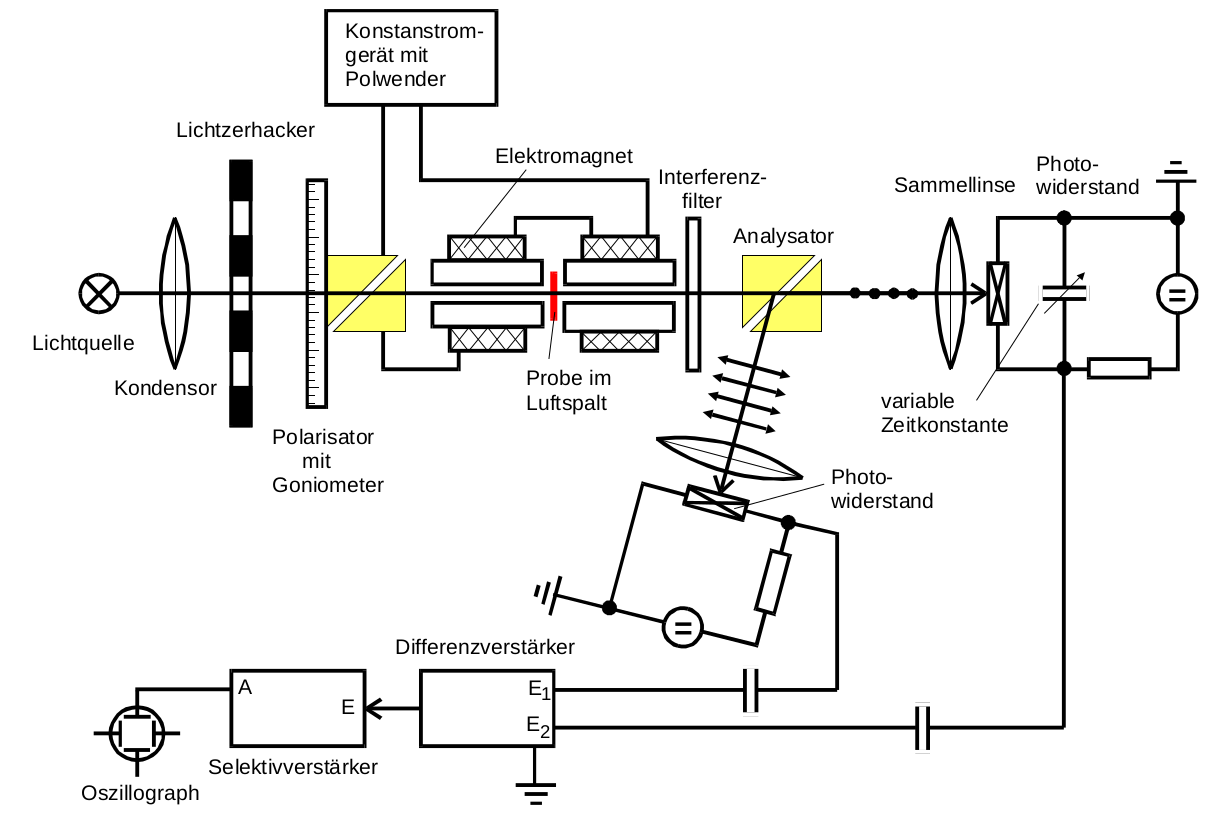
\includegraphics[width=0.8\textwidth]{./Bilder/aufbau.png}
	\caption{Der Versuchsaufbau \cite{man}}\label{fig:aufbau}
\end{figure}

\subsection{Durchführung}
Die beiden Spulen werden hintereinander mit einem konstanten Strom von
$\qty{10}{\ampere}$ versorgt. Eine Hallsonde wird durch die Spule geschoben, um
das maximale Magnetfeld zu messen. Die Proben werden im Versuch in der Mitte
der zwischen den beiden Spulen eingespannt, wo das Magnetfeld am stärksten ist.

Der Faraday Effekt rotiert die Polarisationsebene des Lichtes in der Probe um
den Winkel $\theta$. Um diesen Winkel zu messen wird, das mit einem Goniometer
einstellbare, Glan-Thomson-Prisma gedreht bis die Differenzspannung minimal
ist. Danach wird das Magnetfeld umgepolt und das Signal erneut minimiert.
Dieses wird dann für alle $3$ Galliumarsenid - Proben und für jeweils $9$
verschiedenen Wellenlängen durchgeführt.

\newpage